%!TEX TS-program = Arara
% arara: pdflatex: {shell: yes}
\documentclass[14pt,ngerman]{beamer}

\usepackage[T1]{fontenc}
\usepackage{booktabs}
\usepackage{babel}
\usepackage{graphicx}
\usepackage{csquotes}
\usepackage{xcolor}
\usepackage{tikz}
\usepackage{listings}
\usepackage{bera}
 
\definecolor{colBack}{rgb}{1,1,0.8}
\definecolor{hellgelb}{rgb}{1,1,0.8}
\definecolor{colKeys}{rgb}{0,0,1}
\definecolor{colIdentifier}{rgb}{0,0,0}
\definecolor{colComments}{rgb}{1,0,0}
\definecolor{colString}{rgb}{0,0.5,0}
 
\lstset{%
    float=hbp,%
    basicstyle=\ttfamily\footnotesize, %
    identifierstyle=\color{colIdentifier}, %
    keywordstyle=\color{colKeys}, %
    stringstyle=\color{colString}, %
    commentstyle=\color{colComments}, %
    columns=flexible, %
    tabsize=2, %
    frame=single, %
    extendedchars=true, %
    showspaces=false, %
    showstringspaces=false, %
    numbers=left, %
    numberstyle=\tiny, %
    breaklines=true, %
    backgroundcolor=\color{colBack}, %
    breakautoindent=true, %
    captionpos=b,
    language={[LaTeX]TeX}
}
 

\lstset{literate=%
    {Ö}{{\"O}}1
    {Ä}{{\"A}}1
    {Ü}{{\"U}}1
    {ß}{{\ss}}1
    {ü}{{\"u}}1
    {ä}{{\"a}}1
    {ö}{{\"o}}1
    {~}{{\textasciitilde}}1
}

\author{Uwe Ziegenhagen}
\title{\textit{TikZ}ische Erlebnisse}
\subtitle{Dante Frühjahrstagung 2025}


\begin{document}

\begin{frame}

\maketitle

\end{frame}

\begin{frame}
\frametitle{Über diesen Vortrag}

\begin{itemize}
\item Habe diverse Dinge mit TikZ umgesetzt
\item Erkenntnis: TikZ ist \textit{echt} mächtig 
\item Programm für heute: 
\begin{itemize}
	\item Grundlagen
	\item Beispiele
\end{itemize}

\end{itemize}
\end{frame}

\section{Geschichte und Grundlagen} 

\begin{frame}
\frametitle{Geschichte}

\begin{itemize}
\item TikZ = TikZ ist kein Zeichenprogramm
\item TikZ = \enquote{Frontend} für PGF
\item Entwickler Till Tantau, Christian Feuersänger
\end{itemize}
\end{frame}

\begin{frame}[containsverbatim]
\frametitle{Grundlagen I}

\begin{lstlisting}
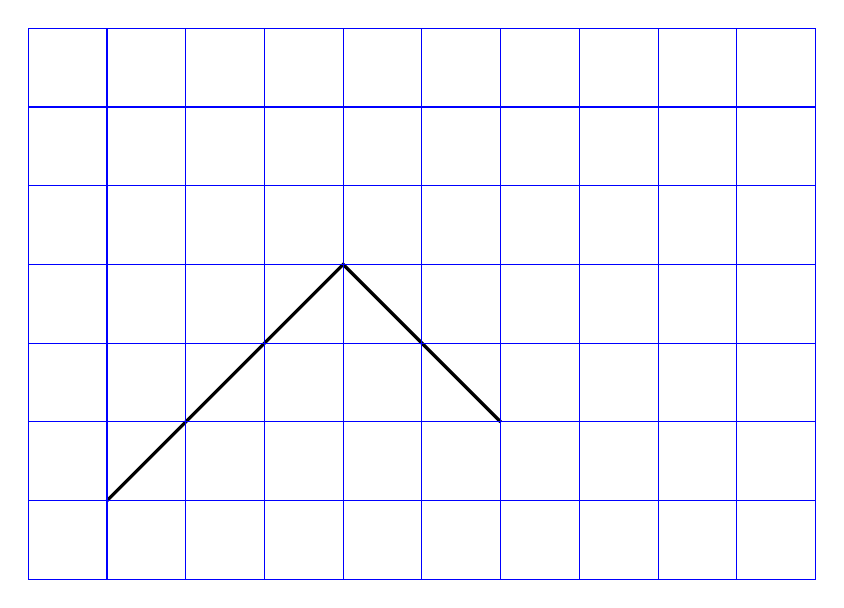
\begin{tikzpicture}
\draw[very thick] (1,1) -- (4,4) -- (6,2);
\draw[step=1cm,blue,thin] (0,0) grid (10,7);
\end{tikzpicture}
\end{lstlisting}


\end{frame}



\begin{frame}[containsverbatim]
\frametitle{Grundlagen I}

\begin{lstlisting}
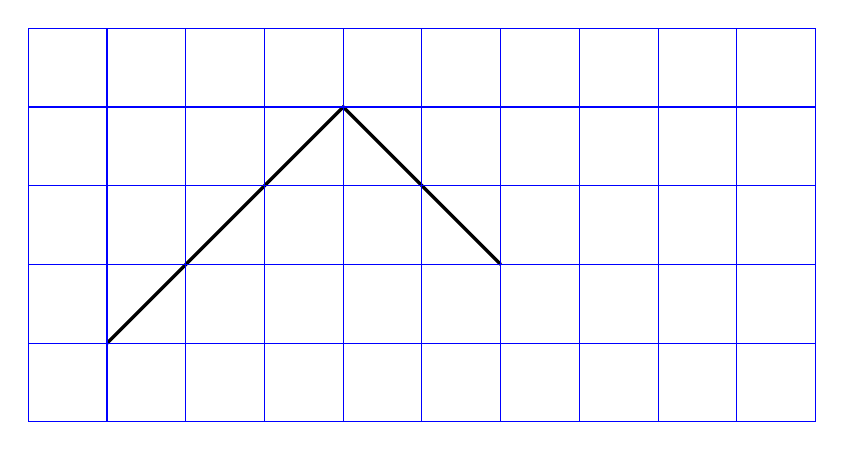
\begin{tikzpicture}
\draw[very thick] (1,1) -- (4,4) -- (6,2);
\draw[step=1cm,blue,thin] (0,0) grid (10,5);
\end{tikzpicture}
\end{lstlisting}

\begin{center}
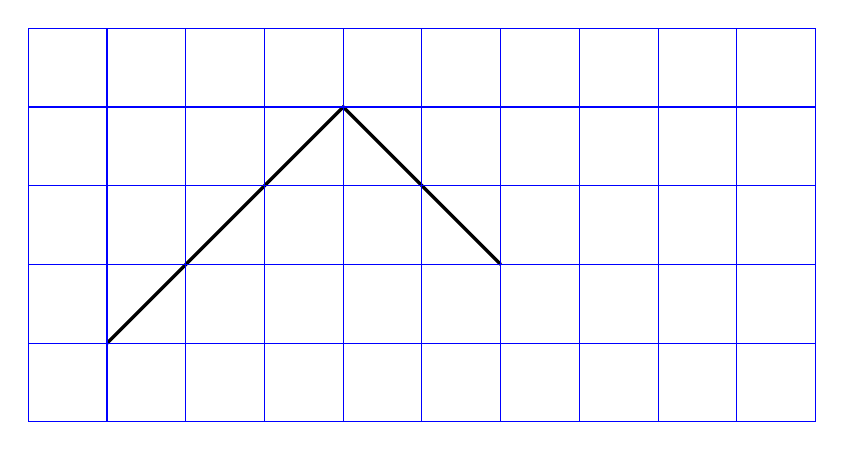
\begin{tikzpicture}
\draw[very thick] (1,1) -- (4,4) -- (6,2);
\draw[step=1cm,blue,thin] (0,0) grid (10,5);
\end{tikzpicture}
\end{center}


\end{frame}


\begin{frame}
\frametitle{Grundlagen I}

\begin{center}
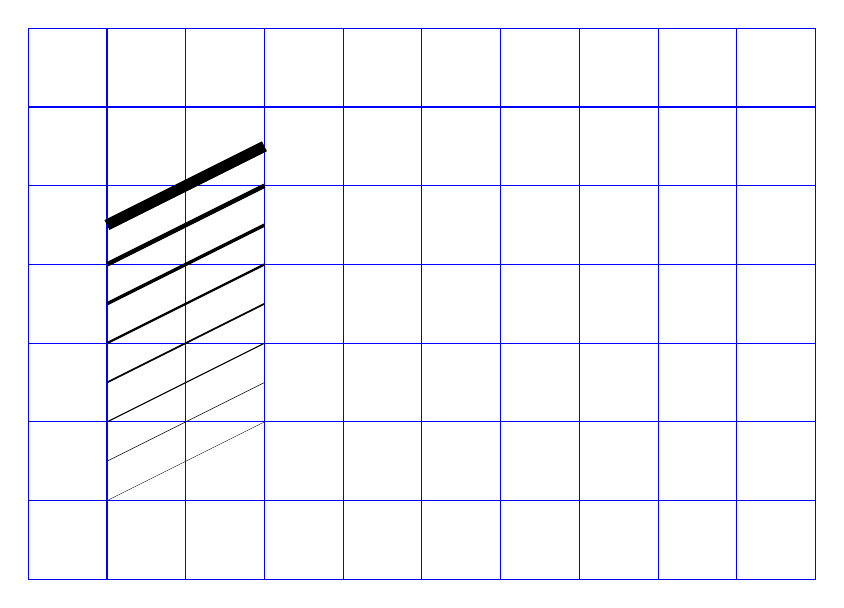
\begin{tikzpicture}
\draw[step=1cm,blue,thin] (0,0) grid (10,7);
\draw[ultra thin] (1,1) -- (3,2);
\draw[very thin] (1,1.5) -- (3,2.5);
\draw[thin] (1,2) -- (3,3);
\draw[semithick] (1,2.5) -- (3,3.5);
\draw[thick] (1,3) -- (3,4);
\draw[very thick] (1,3.5) -- (3,4.5);
\draw[ultra thick] (1,4) -- (3,5);
\draw[line width=4pt] (1,4.5) -- (3,5.5);
\end{tikzpicture}
\end{center}


\end{frame}

\begin{frame}
\frametitle{Grundlagen I}

\begin{center}
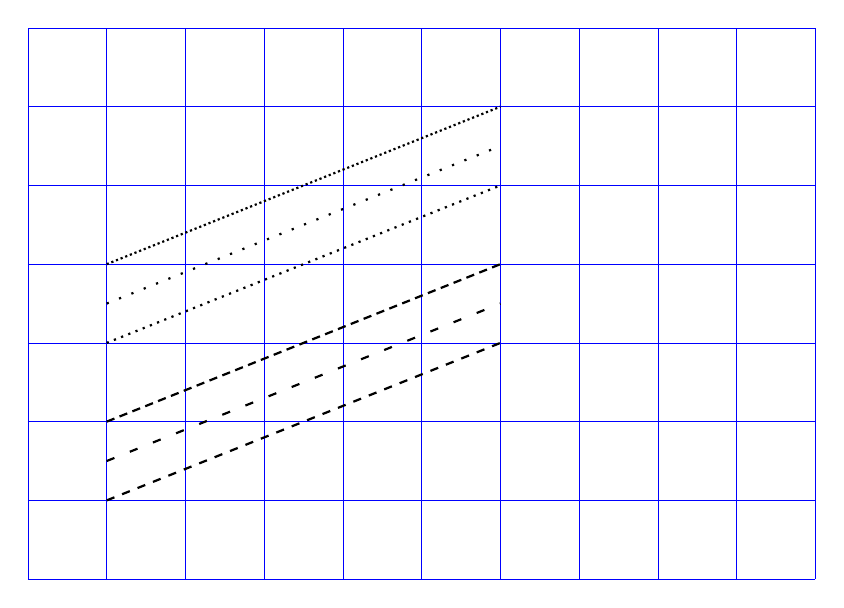
\begin{tikzpicture}
\draw[step=1cm,blue,very thin] (0,0) grid (10,7);

\draw [thick, dashed] (1,1) -- (6,3);
\draw [thick, loosely dashed] (1,1.5) -- (6,3.5);
\draw [thick, densely dashed] (1,2) -- (6,4);
\draw [thick, dotted] (1,3) -- (6,5);
\draw [thick, loosely dotted] (1,3.5) -- (6,5.5);
\draw [thick, densely dotted] (1,4) -- (6,6);
\end{tikzpicture}
\end{center}


\end{frame}



\begin{frame}
\frametitle{Grundlagen III mit Update des Ursprungs}

\begin{center}
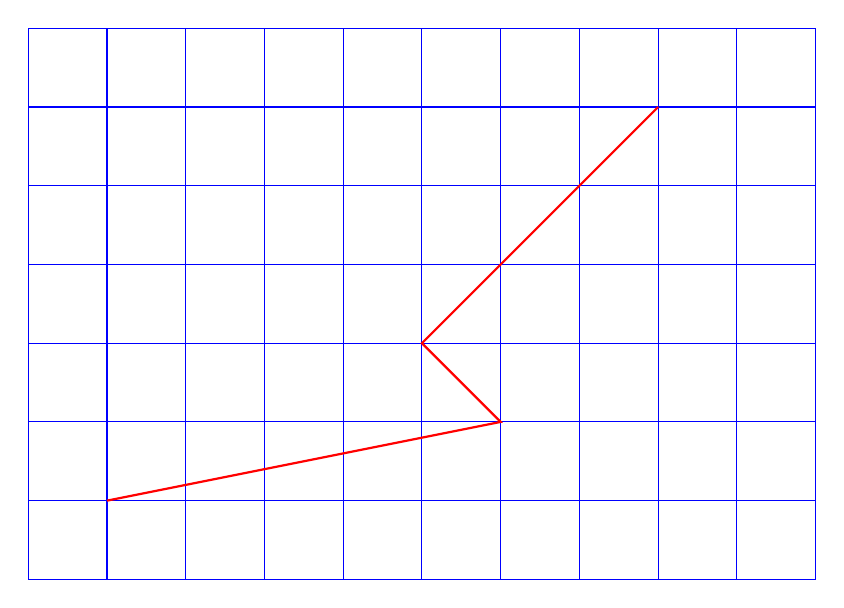
\begin{tikzpicture}
\draw[step=1cm,blue,thin] (0,0) grid (10,7);

\draw[thick, red] (1,1) -- ++(5,1) -- ++(-1,1) -- ++(3,3);
\end{tikzpicture}
\end{center}

\end{frame}


\begin{frame}
\frametitle{Grundlagen III - Koordinaten ohne Update}

\begin{center}
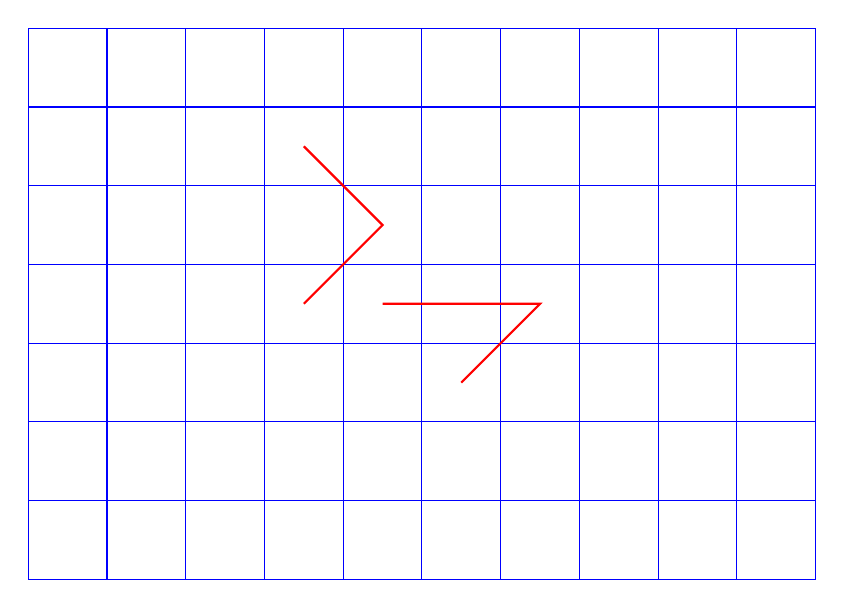
\begin{tikzpicture}
\draw[step=1cm,blue,thin] (0,0) grid (10,7);
\draw[thick, red] (3.5,3.5) -- ++(1,1) -- ++(-1,1);

\draw[thick, red] (5.5,2.5) -- +(1,1) -- +(-1,1);

\end{tikzpicture}
\end{center}

\end{frame}

\begin{frame}
\frametitle{Grundlagen IV -- Polarkoordinaten}

\begin{center}
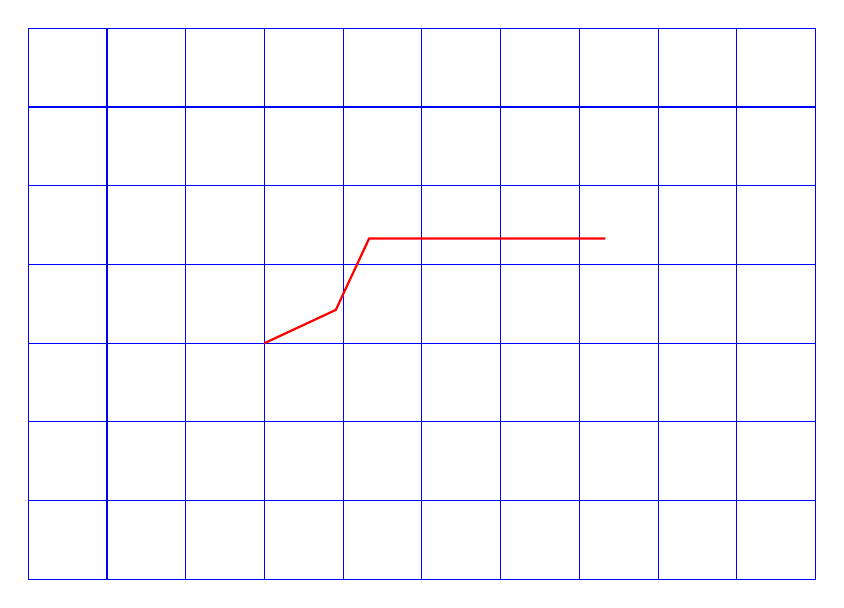
\begin{tikzpicture}
\draw[step=1cm,blue,thin] (0,0) grid (10,7);
\draw[red,thick] (3,3) -- ++(25:1) -- ++(65:1) -- ++(0:3) ;

\end{tikzpicture}
\end{center}

\end{frame}

\begin{frame}
\frametitle{Grundlagen IV}



\end{frame}

\begin{frame}
\frametitle{Grundlagen II}

nodes

\end{frame}


\begin{frame}
\frametitle{Grundlagen II}

Shapes

\end{frame}



\begin{frame}
\frametitle{Grundlagen II}

Shapes Formatieren

\end{frame}



\begin{frame}
\frametitle{Grundlagen II}

Anchors
\end{frame}

\begin{frame}
\frametitle{Anwendungen}


\end{frame}


\end{document}